
\section{Frequentist Inference}

\subsection{Estimators and Sampling Distributions}

Estimators are just functions of random variables. (They are also statistics, because any function of random variablesis a statistic by definition.) Sampling distributions are the distributions of estimators. Usually estimators will be functions of more than one random variable. The canonical example of a sampling distribution is the distribution of the mean (of a sample of independent random variables), and in this case estimator (the sample mean) would typically be estimating the unknown population mean.

Estimators are typically written as the parameter they are estiamting, but with a ``hat''. So the estimators $\hat{\mu}$ and and $\hat{\sigma}$  below, would be estimators of the population mean $\mu$, and population standard error,  $\sigma$, respectively. 

\be
\hat{\mu}\;=\;\bar{y}&=&\frac{\sum_{i=1}^ny_i}{n} \\
\hat{\sigma}&=&\frac{\sum_{i=1}^n(y_i-\bar{y})^2}{(n-1)}
\ee

\noindent
where $y_1,\ldots,y_n$ is the observed data. Notice that $\hat{\mu}$ and $\hat{\sigma}$ are just functions of the random variables (the observed data) $y_1,\ldots,y_n$.

Figure~\ref{fig:samplingdbns} shows the sampling distribution of (a) the sample mean of a random variable $y$, (b) the standard deviation $\hat{\sigma}$, and (c) the \textit{geometric} mean $(\prod_{i=1}^ny_i)^{1/n}$, for samples of size $n=5$. 

\begin{figure}[ht!]
\caption{\small The sampling distribution of (a) the mean of a sample of $y$s, (b) the stanadard deviation $\hat{\sigma}$ of the sample, and (c) the geometric mean $(\prod_{i=1}^ny_i)^{1/n}$, for samples of size $n=5$.}
\centering
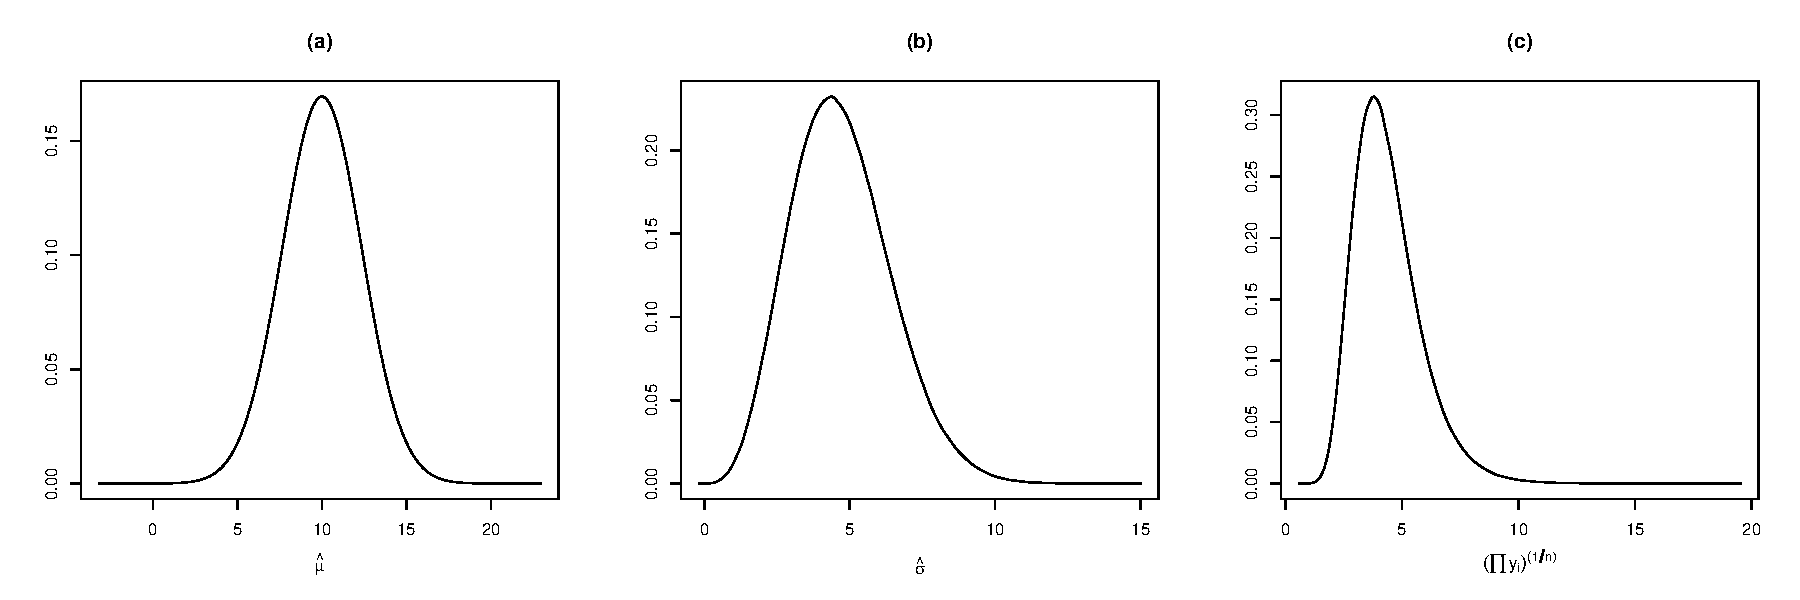
\includegraphics[width=0.9\textwidth]{samplingdbns.pdf}
\label{fig:samplingdbns}
\end{figure}

Sampling distributions depend on the statistic or estimator used (as is apparent from Figure~\ref{fig:samplingdbns}), and on the sample size (5 in this figure). The larger the sample size, the smaller the variance (width) of the sampling distribution.

We use the sampling distribution to get confidence intervals. For example, the point of the estimated sampling distribution of the mean that has 2.5\% of the density to the its left and the point that has 2.5\% to its right constitute the 95\% confidence bounds for the population mean.


\subsection{Estimator Properties}

The two main properties of estimators that we are most often interested in are their bias and their variance. Bias is just the difference between the expected value of the estimator (the mean of its sampling distribution) and the true value:

\be
\mbox{Bias}&=&E(\hat{\theta})-\theta,
\ee

\noindent
where $\hat{\theta}$ is the estimator of $\theta$. The variance of an estimator is the variance of its sampling distribution.

Note that individual estimates will be different from the true value of the parameter they are estimating, because estimators are random variables. The fact that a single estimate is  different from the true value does not mean that the estimator is biased, it is only when the \textit{expected value} of the estimator is different from the true value that we can say that the estimator is biased.

There are many possible estimators of any population parameter. For example, here is the maximum likelihood estimator (MLE) of $\sigma$, which is a little different from the usual estimator $\hat{\sigma}$:

\be
\tilde{\sigma}&=&\frac{\sum_{i=1}^n(y_i-\bar{y})^2}{n}.
\ee

We would like estimators to be unbiased and have low variance. One of the main reasons we use $\hat{\sigma}$ in preference to the MLE $\tilde{\sigma}$ is that $\hat{\sigma}$ is and unbiased estimator of $\sigma$, while $\tilde{\sigma}$ is biased by a factor of $n/(n-1)$.

\subsubsection{Expected values of nonlinear functions of estimators}

The expected value (mean) of a non-linear function of a random varible is \textbf{not} in general equal to the non-linear function of the expected value of the random variable. 

For example, suppose we know that $E(\hat{\theta})=\theta$, so that the random variable $\hat{\theta}$ is an unbiased estimator of $\theta$, but we are really interested in estimating $\exp(\theta)$, not $\theta$:

\be
\mbox{If}\;\;E\left(\hat{\theta}\right)=\theta&\mbox{then}&
E\left(e^{\hat{\theta}}\right)\neq e^{\theta}.
\ee

Because $\exp()$ is a nonlinear function, the expected value of $\exp(\hat{\theta})$ is \textit{not} $\exp(\theta)$, and so $\exp(\hat{\theta})$ is a \textit{biased} estimator of $\exp(\theta)$. This is an important fact that is often overlooked.

\subsection{Maximum Likelihood Estimation}

Suppose we want to estimate some parameter $\theta$ (e.g. the probability of detecting an animal) and we have some data $\bm{y}$ (e.g. the number of animals we detected). To make the example really simple, let's suppose that we also know the number of animals in the population, $N$, to be 100, and the number of detected animals is $y=10$. How would we estimate the detection probability $\theta$ by maximum likelihood?

Here is how we now proceed

\ben

\item \textbf{Get the likelihood function}: After referring to Table~\ref{tab:distributions}, we decide to model the data $y$ using a binomial distribution, and our likelihood function is therefore just the binomial distribution with some unknown $\theta$, evaluated at $y=10$ (with the detection, or ``success'' probability $\theta$ being unknown). We write it as $P(y=10;\theta)$, the ``$;\theta$'' being there just to make the dependence on the parameter $\theta$ explicit.  Because we know $y$, we think of this as a likelihod function that depends on the parameter $\theta$ and so write it as $L(\theta)$:

\be
P(y=10;\theta)\;=\;L(\theta)&=&{100\choose 10}\theta^{10}(1-\theta)^{100-10}.
\label{eq:binlik}
\ee

Figure~\ref{fig:thetalikelihood} shows the likelihood $L(\theta)$ for all values of $\theta$. 

\begin{figure}[ht!]
\caption{\small The likelihood function $L(\theta)$ for observed count $y=10$. The dashed red line shows where the maximum occurs.}
\centering
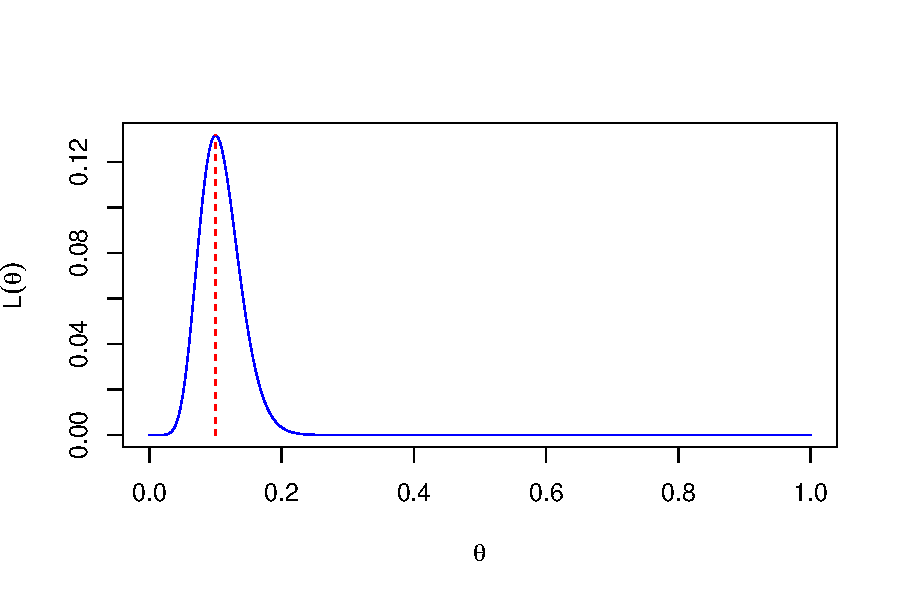
\includegraphics[width=0.55\textwidth]{thetalikelihoodmax.pdf}
\label{fig:thetalikelihoodmax}
\end{figure}

\item \textbf{Find the value of $\theta$ that maximises the likelihood function}. This is the maximum likelihood estimate (MLE). Finding it is just a question of finding the point at which the first derivative (the slope) of the likelihood function is zero and the second derviative (the rate of change of slope) is negative as you move from left to right. (Convince yourself that when the slope is zero, a negative second derivative corresponds to a maximum and a positive second derivative to a minimum of the function.)

Well, actually that is not what we do - we do that for the \textbf{log} of the likelihood function. Why? Because likelhood functions usually contain products of things and when you log the likelihood these become sums of things, and finding derivatives of sums is much easier than fiding derivatives of products. But are we sure that the maximum of the log-likelihood is at the same point as the maximum of the likelihood (I hear you ask)? Yes, because if any function increases, its log also increases, and if it decreases its log also decreases -- so the point at which the function is not increasing or decreasing (slope zero) is the point at which the log of the function is not increasing or decreasing.

By differntiating the log of Eqn~\eqref{eq:binlik} with respect to $\theta$ we find the slope of the log-likelihood, and by setting this slope equation to zero and solving for $\theta$ we find the MLE. (We should also calculate the second derivative and check that it is negative.) For this simple likelihood we can do this algebraically (try it yourself, using the relevant formulae for derivatives from the Maths section of these notes.) The maximum turns out to be at $\theta=y/N=10/100=0.1~$.

\begin{figure}[ht!]
\caption{\small The log-likelihood function $l(\theta)=\log\{L(\theta)\}$ for observed count $y=10$. The dashed red line shows where the maximum occurs.}
\centering
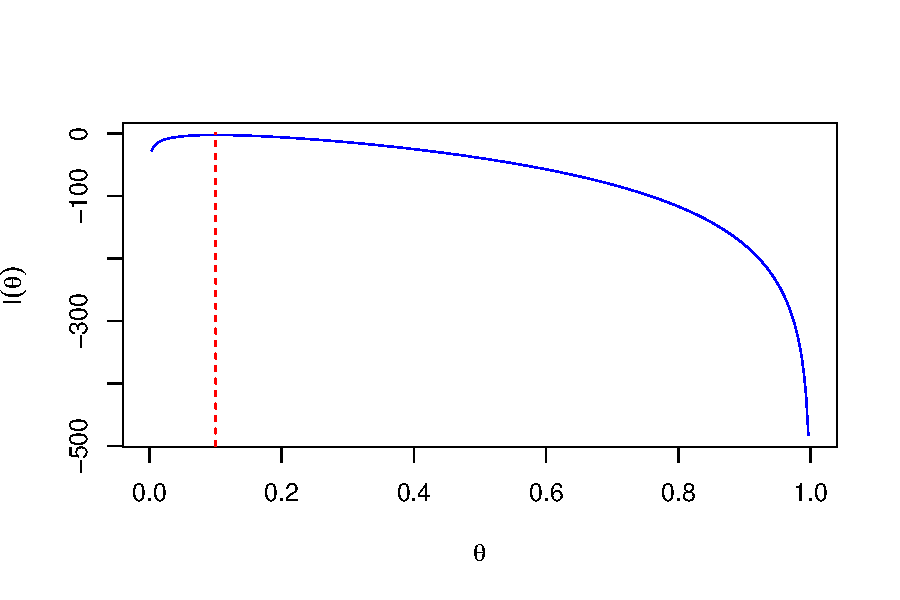
\includegraphics[width=0.55\textwidth]{thetaloglikelihoodmax.pdf}
\label{fig:thetaloglikelihoodmax}
\end{figure}

The maxima of the more complicated likelihood functions that we often have to deal with in realistically complex problems often cannot be found algebraically. In this case we find them by getting a computer to search (in an intelligent way) for the maximum. There are various algorothms for doing this, which we won't go into here.

\item \textbf{Find the sampling distribution of the MLE}. The MLE is just a function of the data (it is $\hat{\theta}=y/N$ in our simple example, where $y$ is the data) and so it has some sampling distribution. But what is its sampling distribution? For most MLEs, we don't actually know, so we usually either approximate the sampling distribution by simulating from our data or from our model using the MLE (bootstrapping), or we rely on powerful asymptotic results that give the sampling distribution of \textbf{any MLE} when sample size is ``large enough'' (strictly when it approaches $\infty$, but in practice for large samples). 

\een


\subsection{MLE Properties}

These are some key properties of MLEs:

\bi

\item MLEs are asymptotically unbiased (as sample size approaches $\infty$), but not necessarily unbiased for small sample sizes.

\item Asymptotically, MLEs have the smallest possible variance among all (asymptotically) unbiased estimators.

\item The sampling distribution of any MLE is (asymptotically, as sample size approaches $\infty$) normal, with mean equal to the true value of the parameter being estimated, and with variance equal to the inverse of the second derivative of the log-likelihood function (i.e., the inverse of the rate of change of the slope) at the MLE.

\item MLEs are ``invariant'', which means that the MLE of a function of an estimator is the function of the MLE. For example, we know that asymptotically, the sampling distribution of $\hat{\mu}$ is normal. Then (rather counter-intuitively) the sampling distributions of functions of $\hat{\mu}$ like $\exp(\hat{\mu})$ and $\sqrt{\hat{\mu}}$ are also asymptotically normally distributed, even though they are not normally distributed for finite sample size.
\ei
